% =====================================================================
% 4. Simulações computacionais
% Imagens geradas com o código do projeto (script descartável chamando renderizar_cena_completa).
% Tempos medidos em macOS, Python 3.14, numpy 2.5.5, matplotlib 3.11.2, scikit-image 0.26.0.
% Pendência: refazer as imagens e os tempos se o código do pipeline mudar.
% =====================================================================
\section{Simulações computacionais}\label{sec:simulacoes}

As simulações foram feitas em Python 3.14, com NumPy, Matplotlib e scikit-image. A malha de cada
objeto foi gerada com 80 pontos por eixo. A câmera principal usa $eye = (9{,}75;\ 13;\ 6{,}5)$,
$at = (0, 0, 0)$ e $up = (0, 1, 0)$, e a luz fica em $(5;\ 20;\ 15)$.

\subsection{Três resoluções}\label{sec:sim-resolucoes}

A Figura~\ref{fig:resolucoes} mostra a mesma cena rasterizada em $200 \times 200$, $400 \times 400$
e $800 \times 800$ pixels. Com mais pixels, os contornos ficam mais lisos e o brilho especular
aparece com mais detalhe. Em $200 \times 200$ já dá para reconhecer os objetos, mas as bordas
ficam serrilhadas. O tempo de rasterização foi de 0,8 s, 0,9 s e 1,4 s, respectivamente, sem contar
a geração das malhas, que levou 0,2 s. A cena tem 62\,452 triângulos. Nenhum ficou fora do volume
de visão, 32\,204 foram descartados por estarem de costas e 30\,248 foram desenhados.

\begin{figure}[H]
  \centering
  \caption{Cena rasterizada em três resoluções}\label{fig:resolucoes}
  \begin{subfigure}{0.31\textwidth}
    \centering
    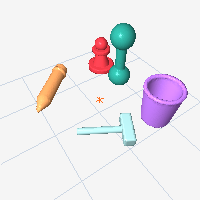
\includegraphics[width=\textwidth]{04-simulacoes/eye1-200.png}
    \caption{$200 \times 200$}
  \end{subfigure}\hfill
  \begin{subfigure}{0.31\textwidth}
    \centering
    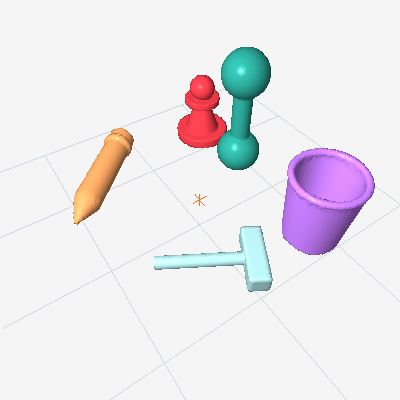
\includegraphics[width=\textwidth]{04-simulacoes/eye1-400.png}
    \caption{$400 \times 400$}
  \end{subfigure}\hfill
  \begin{subfigure}{0.31\textwidth}
    \centering
    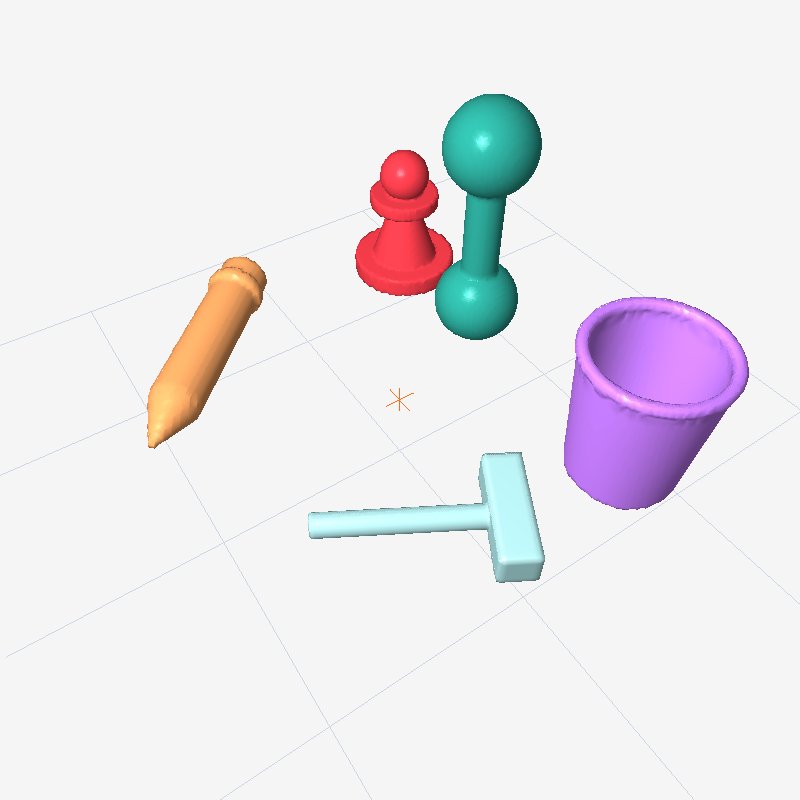
\includegraphics[width=\textwidth]{04-simulacoes/eye1-800.png}
    \caption{$800 \times 800$}
  \end{subfigure}
  \fonte{Os autores (2026).}
\end{figure}

\subsection{Mudança do eye}\label{sec:sim-eye}

Quando o \textit{eye} muda para $(26;\ 18;\ 28)$, o código recalcula a base da câmera e a matriz de
visualização, e a imagem muda. Nessa posição, a câmera fica mais longe e mostra todos os objetos
(Figura~\ref{fig:eye2}).

\figura{04-simulacoes/eye2-400.png}{0.45\textwidth}{Cena vista de $eye = (26;\ 18;\ 28)$, em $400 \times 400$}{fig:eye2}{Os autores (2026)}
